\section{What this paper does not claim}\label{supp:notclaimed}

The benchmark is sharp precisely because its scope is narrow, and stating the boundaries
keeps the result from being read wider than the evidence carries it. We do not claim to
recover a program's semantics from scratch. The study measures whether an explanation names
the true causes and regenerates the behavior on a machine whose answer is already known; it
does not show that any method discovers the meaning of a routine without that ground truth in
hand, and the residual that faithfulness alone leaves behind, the gap between the wiring and
the computation, is the point rather than a result to be explained away.

We do not evaluate learned agents. The subject throughout is the bit-exact VCS itself, and
the candidate causes are its registers, RAM cells, and program variables, not the weights of
a trained policy. The neural-network parallels drawn in the discussion and in
Fig.~\ref{supp:fig:repmap} are documented analogues from the literature, not claims proven on
this benchmark; we label them as such so that a reader does not take a mapped failure mode
for a demonstrated one.

We do not prove that neural-network interpretability is impossible. The VCS gap is a
necessary-condition stress test: a method that fails to recover the wiring of a fully known
machine cannot be trusted to recover it on an unknown one, but a method that succeeds here is
not thereby certified on networks. The ``floor'' framing is an evidence-transfer argument,
not a proven lower bound on neural-network interpretability.

We do not measure human plausibility. The plausibility axis is a documented
method-tradition proxy, computed from a fixed rubric rather than collected from raters, and
we report it as a proxy throughout; its job is to expose the danger zone where a convincing
explanation is unfaithful, not to stand in for a human-subjects study. We also do not
redistribute the ROMs: the substrate is validated against an external reference, the records
are reproducible from committed artifacts without the ROMs, and the ROM provenance is given
as hashes so a third party supplies their own legally obtained copies.

\begin{figure}[t]
\centering
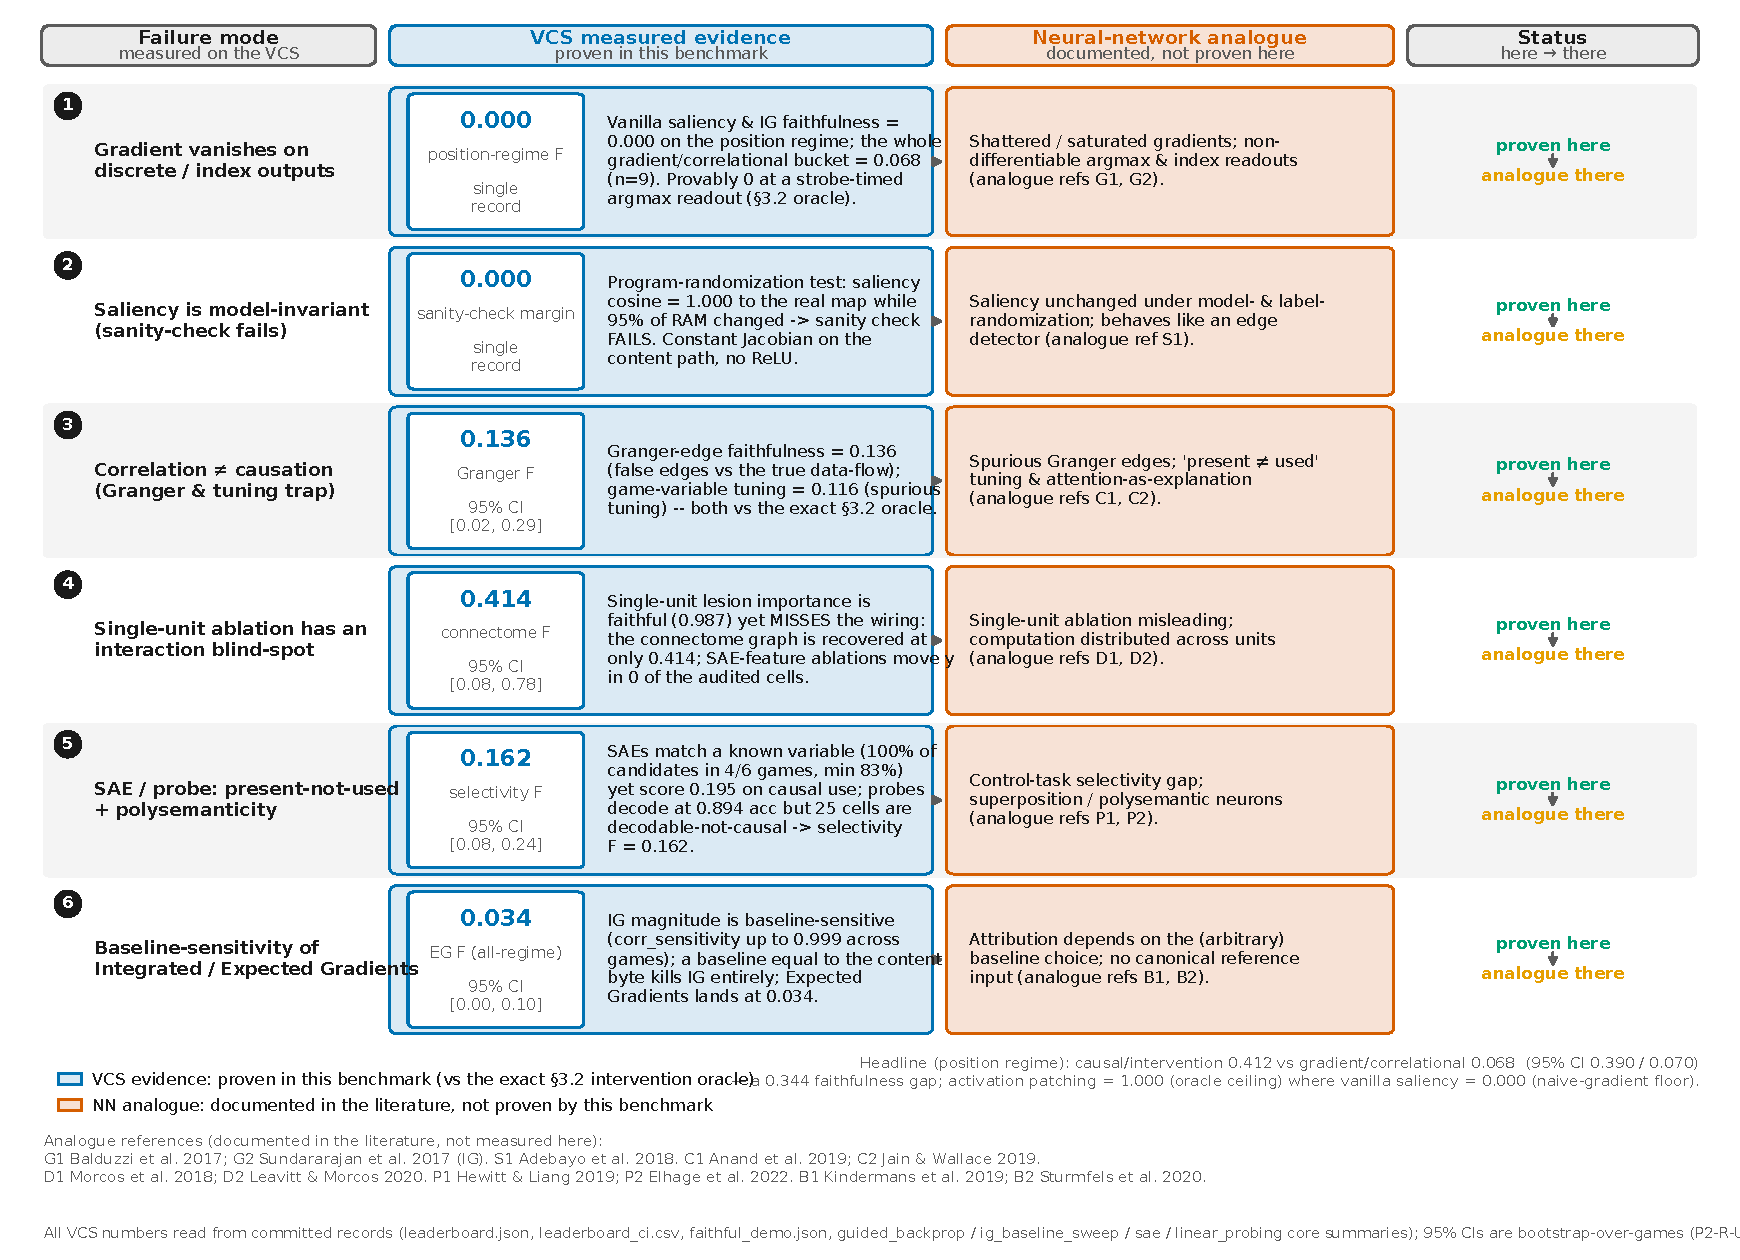
\includegraphics[width=\textwidth]{../figures/fig5_representativeness_map_full.pdf}
\caption{\textbf{Full VCS-to-NN representativeness map.} The full-density version of the
main-text map (Fig.~\ref{fig:representativeness}): each VCS failure mode is placed against its documented
neural-network analogue from the literature. The neural-network column records documented
analogues, not parallels proven by this benchmark; the oracle is the intervention oracle of
\Sectionname3.2, and the underlying per-method values trace to
\texttt{compare/out/leaderboard.json} via Sec.~\ref{supp:provenance}. Note that this full
map is the figure the simplified main-text version condenses.}
\label{supp:fig:repmap}
\end{figure}

\begin{figure}[t]
\centering
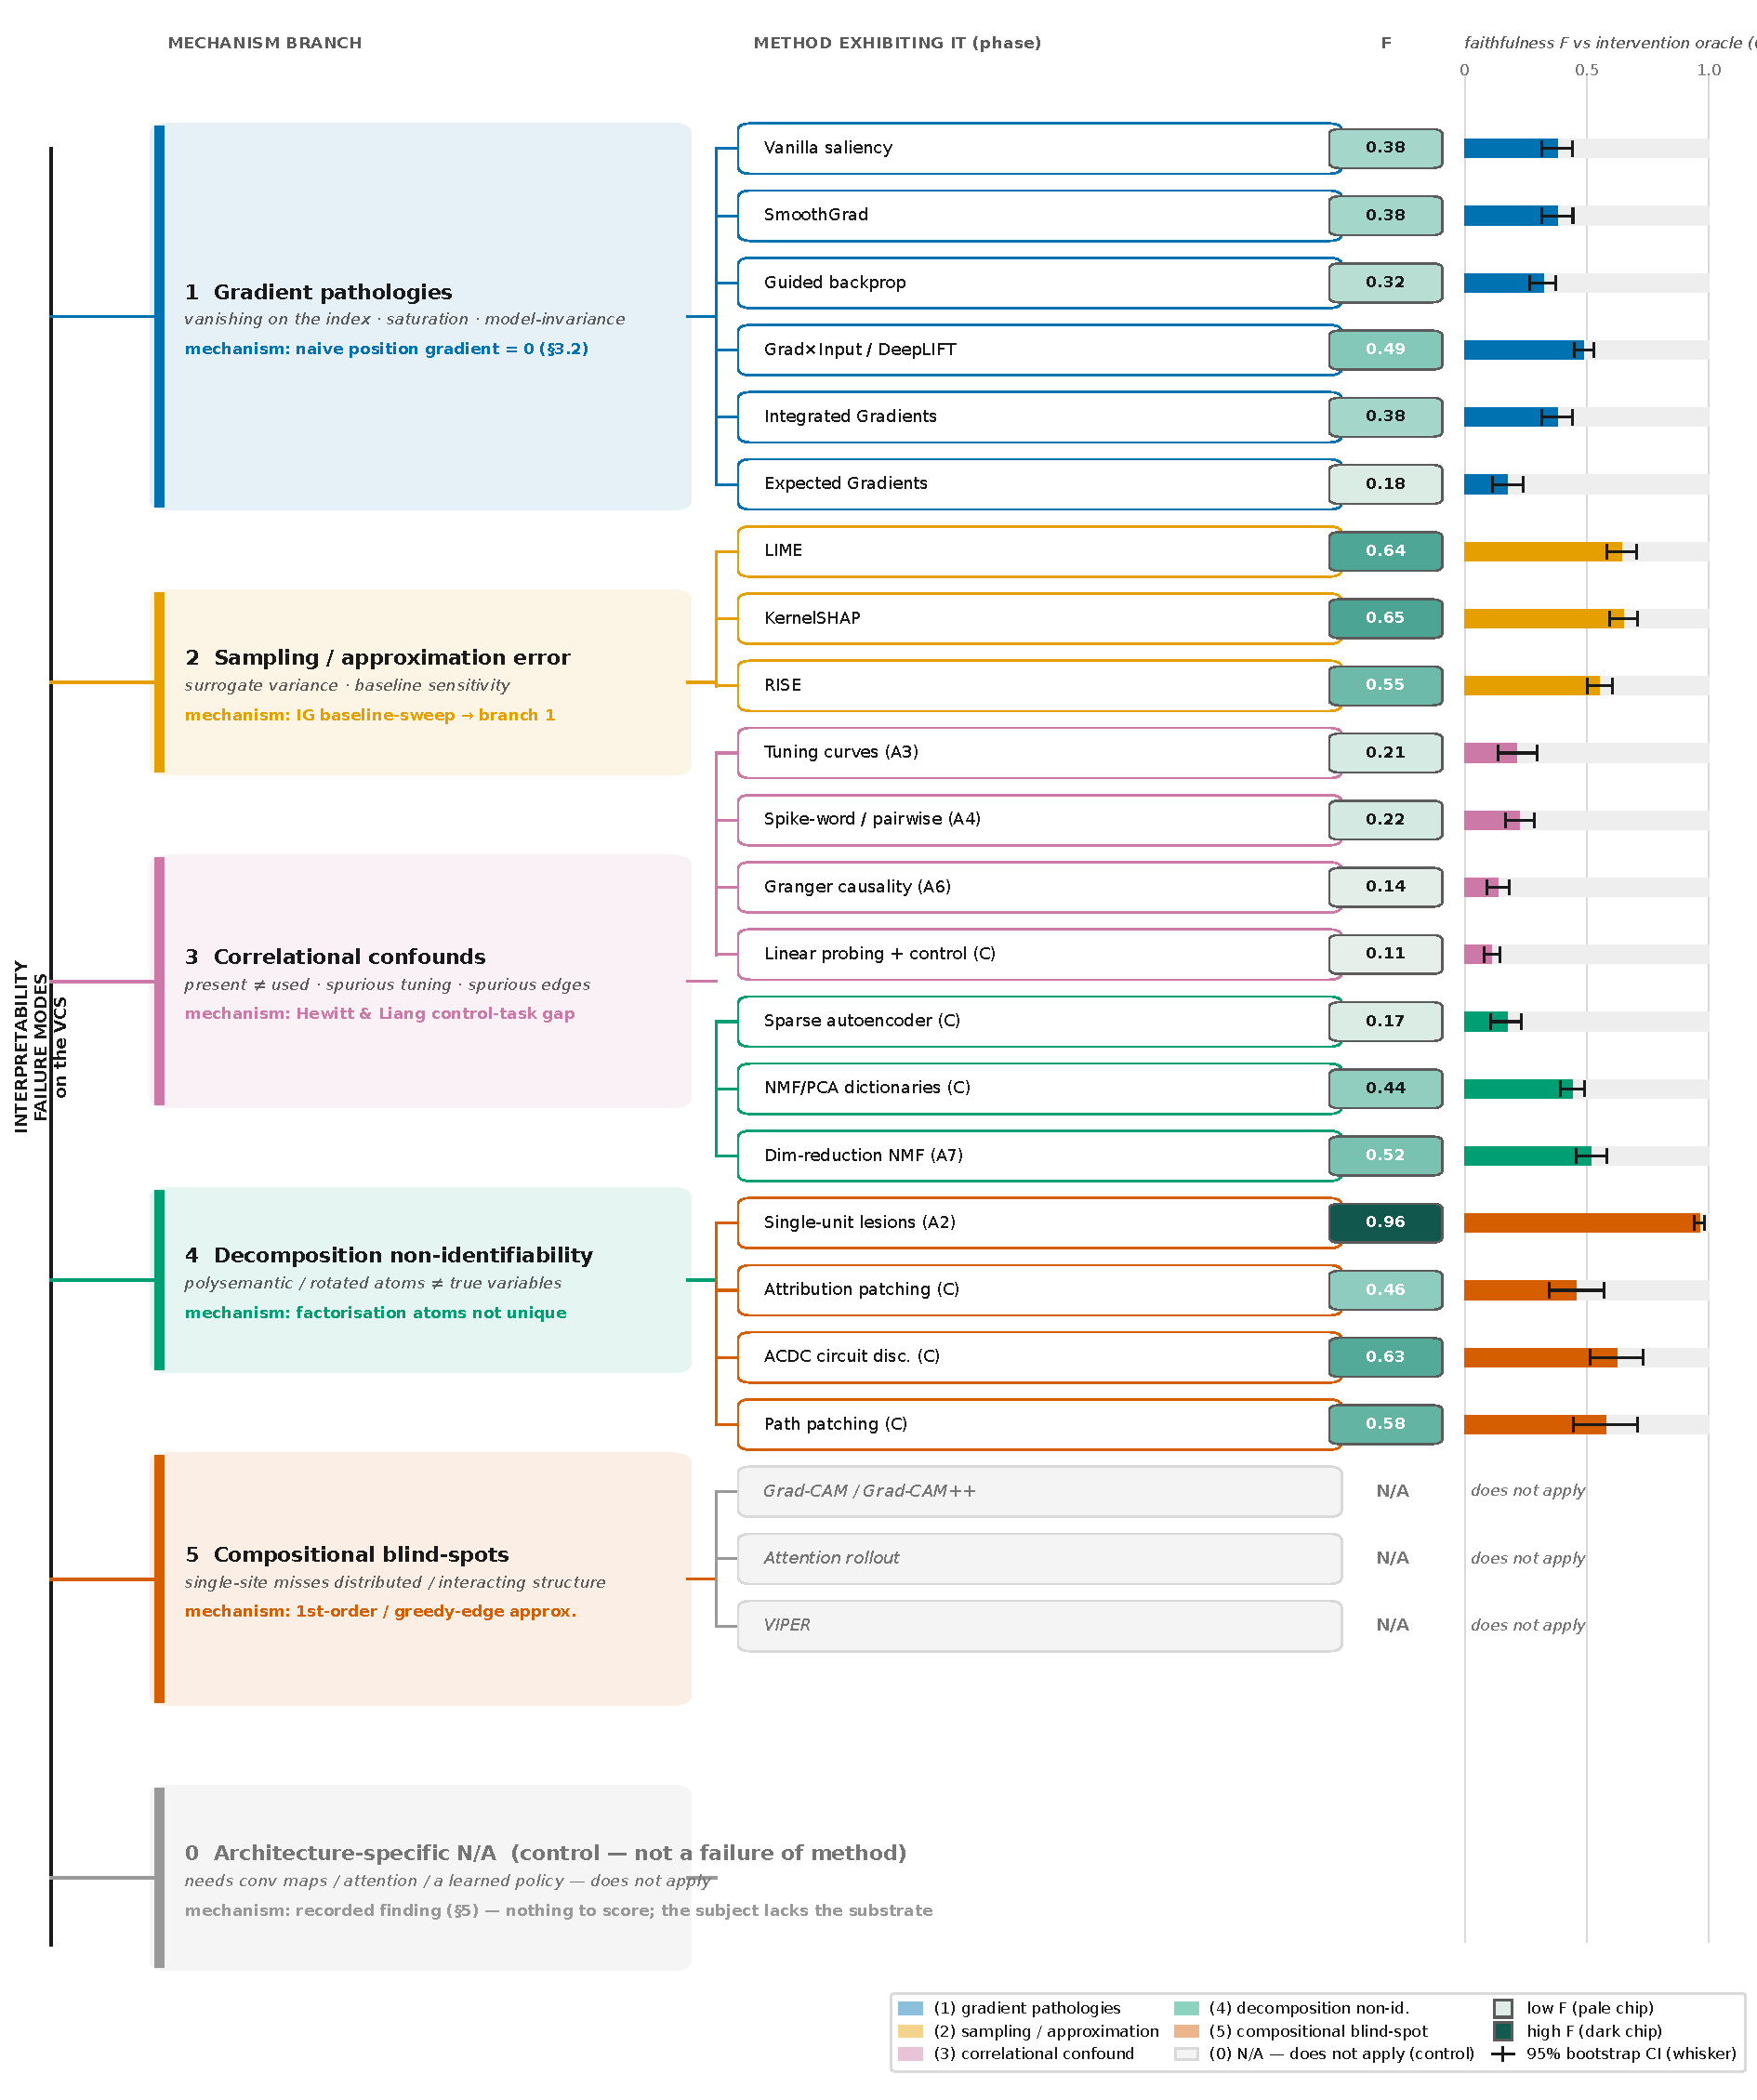
\includegraphics[width=\textwidth]{../figures/fig6_failure_taxonomy_full.pdf}
\caption{\textbf{Full failure taxonomy.} The full-density version of the main-text taxonomy
(Fig.~\ref{fig:taxonomy}): the families of interpretability failure observed on the machine, each annotated
with its faithfulness against the intervention oracle (\Sectionname3.2), reported as $F$ with its
$95\%$ bootstrap confidence interval. The leaf values trace to
\texttt{compare/out/leaderboard.json} and \texttt{leaderboard\_ci.csv} via
Sec.~\ref{supp:provenance}. Note that the gradient and correlational branches collapse on
the discrete position regime, where the naive gradient is provably zero (Prop.~\ref{prop:zero}).}
\label{supp:fig:taxonomy}
\end{figure}
